\documentclass[11pt,letterpaper,titlepage]{article}
\usepackage{fancyhdr}
\usepackage[left=0.75in, right=0.75in, bottom=1.0in]{geometry}
\usepackage{lastpage}
\usepackage{titleref}
\usepackage{booktabs}
\usepackage{appendix}
\appendixtitleon
\appendixtitletocon

\makeatletter

%================== List of figures and tables mods
\usepackage{tocloft}
\usepackage[labelfont=bf]{caption}

\renewcommand{\cftfigpresnum}{Figure\ }
\renewcommand{\cfttabpresnum}{Table\ }

\newlength{\mylenf}
\settowidth{\mylenf}{\cftfigpresnum}
\setlength{\cftfignumwidth}{\dimexpr\mylenf+1.5em}
\setlength{\cfttabnumwidth}{\dimexpr\mylenf+1.5em}



%=================== Graphics
\usepackage{graphicx}
\usepackage[breakwords]{truncate}
\usepackage{float}
\usepackage{array}
\usepackage{amsmath}
\usepackage{mdframed}
\usepackage{fancyvrb}
\usepackage{float}
\usepackage{cancel}
\usepackage{amssymb}
\graphicspath{ {images/} }
\usepackage[usenames,dvipsnames,svgnames,table]{xcolor}
\usepackage[defaultlines=2,all]{nowidow}
\usepackage{listings}
\usepackage{color}
\definecolor{Brown}{cmyk}{0,0.81,1,0.60}
\definecolor{OliveGreen}{cmyk}{0.64,0,0.95,0.40}
\definecolor{CadetBlue}{cmyk}{0.62,0.57,0.23,0}
\usepackage{pdflscape}
\usepackage{relsize}
\usepackage{verbatim}


%=================== Settings
\renewcommand{\baselinestretch}{1.2}
\definecolor{gray}{rgb}{0.4 0.4 0.4}
\newcommand{\stimes}{{\times}}

\begin{document}
\newcommand{\NSCDOCNUMBR}{NSC-REP-15-X}         %Put document number here
\newcommand{\NSCDOCSUBJT}{TECHNICAL REPORT: }   %Put document subject here
\newcommand{\NSCDOCTITLE}{Heat conduction for Unstructured Meshes implemented in $JIC^{Lib2}$}       %Put document title here
\newcommand{\NSCDOCDATE} {March, 2016}    %Put document date here
\newcommand{\NSCDOCREV}  {Rev 1} %Put revision number here

\lstset{language=C++,frame=ltrb,framesep=4pt,basicstyle=\linespread{0.8} \small,
	keywordstyle=\ttfamily\color{OliveGreen},
	identifierstyle=\ttfamily\color{CadetBlue}\bfseries,
	commentstyle=\color{Brown},
	stringstyle=\ttfamily,
	showstringspaces=ture }


%################################# TITLE PAGE ########################
\begin{titlepage}
	\pagestyle{fancy}
	\vspace*{1.0cm}
	\centering
	%\includegraphics{NSC_Logo} \par
	\vspace{1cm}
	%\centering
	%{\Large\bfseries  \NSCDOCNUMBR   \par}
	\vspace{.25cm}
	%\centering
	{\Large\bfseries  \NSCDOCSUBJT \par} 
	{\Large\bfseries \NSCDOCTITLE  \par}
	\vspace{1cm}
	{\Large \NSCDOCDATE \par}
	\vspace{1.0cm}
	{\Large Jan Vermaak \par}
	{\Large \NSCDOCREV \par}
		
	\begin{comment}
	\renewcommand{\arraystretch}{2.0}
	\begin{tabular}{| m{2.5cm} | m{4.5cm} | m{4.5cm} |}
		\cline{2-3}
		\multicolumn{1}{c|}{} & \bfseries{Name} & \bfseries{Signature \& Date} \\ \hline
		\bfseries{Prepared} &     &     \\ \hline
		\bfseries{Reviewed} &     &     \\ \hline
		\bfseries{Reviewed} &     &     \\ \hline
	    \bfseries{Approved} &     &     \\ \hline
	\end{tabular} \par
	\end{comment}
	\vspace{2cm}
	%NSC-FRM-15-1 Rev.1
\end{titlepage}


\pagestyle{fancy}
\rfoot{Page \thepage \ of \pageref{LastPage}}
%\cfoot{NSC-FRM-15-1 Rev.1}
\cfoot{}
\lfoot{\truncate{14cm}{\NSCDOCTITLE}}
\rhead{}
\chead{\currentname}
\lhead{}
\renewcommand{\footrulewidth}{0.4pt}
\tableofcontents
\addtocontents{toc}{~\hfill\textbf{Page}\par}

\listoffigures
\listoftables
\chead{Contents}


\newpage
\chead{1 Derivation of the general Heat Conduction Equation}
\section{Derivation of the general Heat Conduction Equation}
The heat conduction equation follows the basic thermodynamic law of conservation of energy $E$. This means that energy coming into a control volume, $E_{in}$, must equal the amount energy stored within the control volume, $E_{store}$, plus the energy leaving the system, $E_{out}$. So, as an equation this looks like:
$$
	 E_{store} = E_{in}-E_{out}
$$
\begin{center}
	\begin{minipage}[c]{0.6\textwidth}

		\begin{figure}[H]
		
			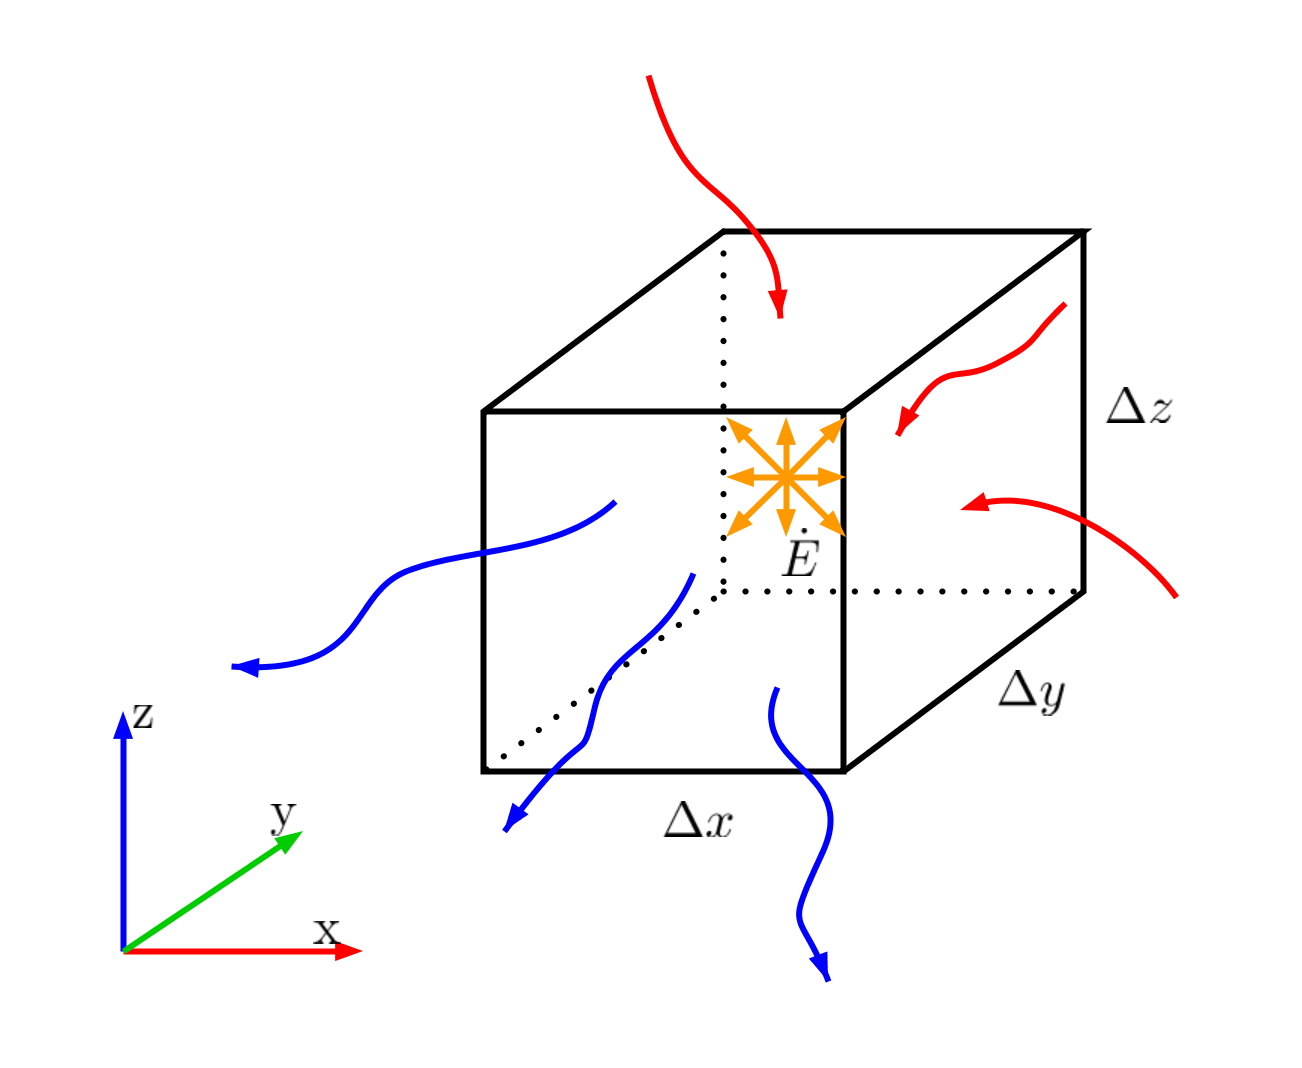
\includegraphics[width=4.0in]{FiniteCube.png}
			\caption{Simple control volume for a structured mesh.}
			\label{figure:SimpleControlVolume}
		\end{figure}
	\end{minipage}
\end{center}
\bigskip
This equation now forms a basis from which we can derive more detailed physical representations. For a visual representation see Figure . We begin by defining the \textbf{heat capacity}, $C$, of a material which can be used as a measure of the material's internal energy. Technically there is a little bit more that goes into internal energy, but for solids we can approximate the energy storage behavior very accurately by using the \textbf{constant pressure} heat capacity, $C_p$ \textcolor{red}{(Justification needed for this assumption)}. The heat capacity of a solid material as defined as the energy, $E$ (in Joules), that is stored in the material per unit mass, $m$ (in kilograms), and per unit temperature, $T$ (in Kelvin). As an equation, this looks like this:
\newline
\begin{equation}
C_p=\frac{E}{\Delta m.T}
\end{equation}
\newline
Now in the absence of a non-solid material adjacent to the control volume in question we can regard the incident or escaping energy to only occur due to heat conduction. This heat conduction at the control volume surfaces is governed by the following equation:
\newline
\begin{equation}
\dot{Q}=-\hat{n} \cdot kA\frac{dT}{dx}
\end{equation}
\newline
Where $\hat{n}$ is the surface normal,$\dot{Q}$ is the heat transfer rate (in $J.s^{-1}$ or $W$), $k$ is the material's thermal conductivity ($W.m^{-1}.K^{-1}$), $A$ is the heat transfer area and $x$ is direction in which the derivative is defined. For a structured mesh, where the normals have been included for the forward and the aft positions along te control volume boundary, this can be written as:
\newline
\begin{equation}
\begin{aligned}
\dot{Q}_{net}= & \ (-k\Delta y \Delta z\frac{dT}{dx})_{aft} \ - \ (-k\Delta y \Delta z\frac{dT}{dx})_{fwd} \\
             + & \ (-k\Delta x \Delta z\frac{dT}{dy})_{aft} \ - \ (-k\Delta x \Delta z\frac{dT}{dy})_{fwd} \\
             + & \ (-k\Delta x \Delta y \frac{dT}{dz})_{aft} \ - \ (-k\Delta x \Delta y \frac{dT}{dz})_{fwd}
\end{aligned}
\end{equation}
\newline
Finally, we can account for the energy generated within the control volume, $\dot{E}_{gen}$, by electric resistance, electromagnetic heating or nuclear fission. After putting all of this into the energy conservation equation, we obtain:
\begin{equation}
\begin{aligned}
\frac{dE}{dt}=0= & \ \frac{d}{dt} \ \Delta m.C_p.T \\
			   + & \ (-k\Delta y \Delta z\frac{dT}{dx})_{aft} \ - \ (-k\Delta y \Delta z\frac{dT}{dx})_{fwd} \\
	           + & \ (-k\Delta x \Delta z\frac{dT}{dy})_{aft} \ - \ (-k\Delta x \Delta z\frac{dT}{dy})_{fwd} \\
	           + & \ (-k\Delta x \Delta y \frac{dT}{dz})_{aft} \ - \ (-k\Delta x \Delta y \frac{dT}{dz})_{fwd} \\
	           + & \ \dot{E}_{gen}		       
\end{aligned}
\end{equation}
Dividing by the unit volume, $\Delta x \Delta y \Delta z$, we can define the following:
$$
\rho = \frac{\Delta m}{\Delta x \Delta y \Delta z}
$$
$$
\dot{e}_{gen}=\frac{\dot{E}_{gen}}{\Delta x \Delta y \Delta z}
$$
To write:
\begin{equation*}
\begin{aligned}
\frac{dE}{dt}=0= & \ \frac{d}{dt} \ \rho.C_p.T \\
			   + & \ (-k\frac{1}{\Delta x}\frac{dT}{dx})_{aft} \ - \ (-k\frac{1}{\Delta x}\frac{dT}{dx})_{fwd} \\
	           + & \ (-k\frac{1}{\Delta y}\frac{dT}{dy})_{aft} \ - \ (-k\frac{1}{\Delta y}\frac{dT}{dy})_{fwd} \\
	           + & \ (-k\frac{1}{\Delta z} \frac{dT}{dz})_{aft} \ - \ (-k\frac{1}{\Delta z} \frac{dT}{dz})_{fwd} \\
	           + & \ \dot{e}_{gen}		       
\end{aligned}
\end{equation*}
\newline
In this equation, the difference of the forward and aft terms take the form of:
$$
\frac{d}{dx}\approx \frac{f(x+\Delta x)-f(x)}{\Delta x}
$$
And therefore if the mesh is sufficiently small to capture the gradient of the temperature with minimal error, we can write:
\begin{equation*}
\begin{aligned}
\frac{dE}{dt}=0= & \ \frac{d}{dt} \ \rho.C_p.T + \frac{d}{dx}(-k\frac{dT}{dx}) + \frac{d}{dy}(-k\frac{dT}{dy}) + \frac{d}{dz}(-k\frac{dT}{dz}) + \dot{e}_{gen}     
\end{aligned}
\end{equation*}
\newline
And finally, by replacing the derivative collection $\frac{d}{dx}+\frac{d}{dy}+\frac{d}{dz}$ by the coordinate system independent operator, $\nabla$, we get the \textbf{general form of the heat conduction equation}:
\newline
\begin{equation}
\begin{aligned}
 \ \rho.C_p \frac{dT}{dt} - \nabla \cdot (k \nabla T) + \dot{e}_{gen} =0
\end{aligned}
\label{equation:genHeatCon}
\end{equation}
\newline
This equation, although in general form, is still in derivative form. When considering a finite volume approach to meshing, this equation is somewhat hard to transform. In this regard, we need to look at the integral from of the diffusion equation. Specifically we will immediately commence with the use of a truncated octahedron.

\newpage
\chead{2 Derivation of the integral form of the Heat Conduction Equation}
\section{Derivation of the integral form of the Heat Conduction Equation}
\begin{center}
	\begin{minipage}[c]{0.6\textwidth}
		\centering
		\begin{figure}[H]
		
			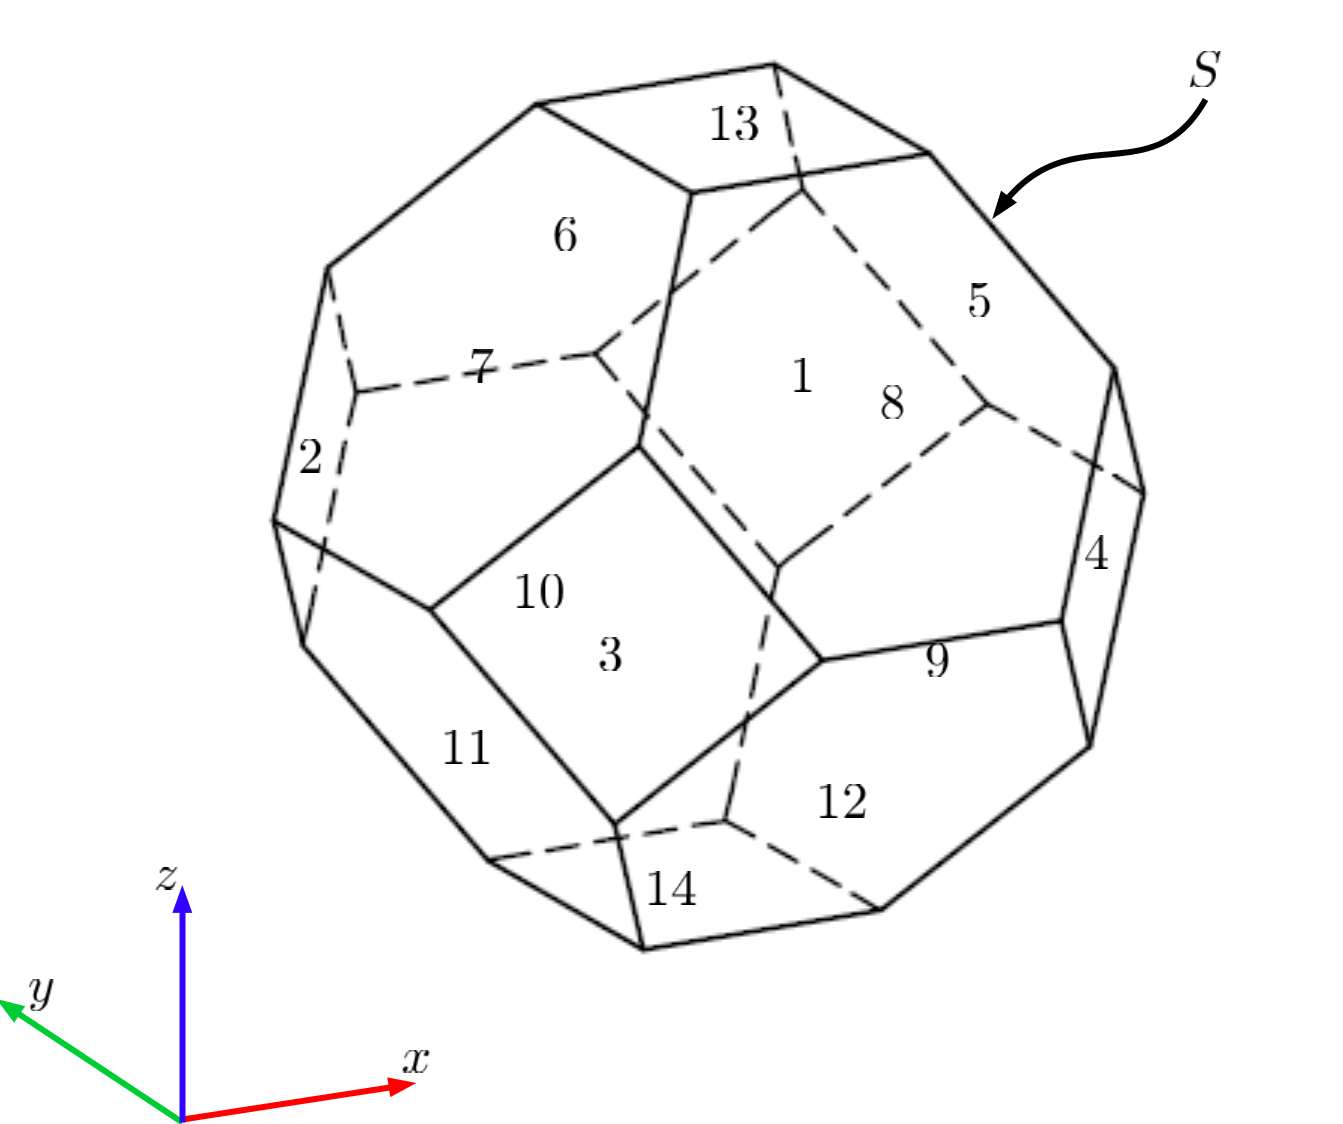
\includegraphics[width=4in]{OctahedronNumbers.png}
			\caption{Numbering scheme for octahedron surfaces.}
			\label{figure:OctahedronNumbers}
		\end{figure}
	\end{minipage}
\end{center}
For a volume filling mesh cell, consider the truncated octahedron cell geometry shown in Figure \ref{figure:OctahedronNumbers}. Our goal is to derive an equation equivalent to eq \ref{equation:genHeatCon} but in integral form. First we start with the heat fluxes at all the faces:

\begin{equation*}
\dot{Q}=-\int_S k\cdot \frac{dT}{dl}.dS
\end{equation*}
\newline
This equation represents the integral of the heat flux over all surfaces. For a finite volume representation we can rewrite this as the sum of all the heat fluxes:

\begin{equation*}
\dot{Q}=\sum_{s=1}^{14} \biggr( -k.A_i.\frac{dT}{dl_{i\to j}}\biggr)
\end{equation*}
\newline
The other terms of the heat conduction are as before and therefore we can write:
\newline
\begin{equation}
\begin{aligned}
 \ \rho.C_p. \frac{dT}{dt} - \sum_{s=1}^{14} \biggr( k.A_i.\frac{dT}{dl_{i\to j}}\biggr) + \dot{e}_{gen} =0
\end{aligned}
\label{equation:finVolHeatCon}
\end{equation}
\newline
At this point it is worth clarifying the definition of $\frac{dT}{dl_{i\to j}}$ which is the derivative of the temperature between two mesh item_id as shown in the figure below:
\begin{center}
	\begin{minipage}[c]{0.5\textwidth}
		\centering
		\begin{figure}[H]
		
			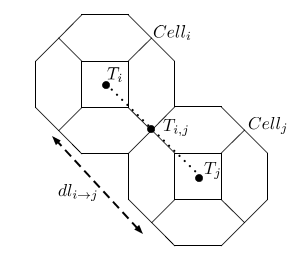
\includegraphics{AdjacentCells2.png}
			\caption{Notations involved with adjacent item_id.}
			\label{figure:Adjacentcells}
		\end{figure}
	\end{minipage}
\end{center}

\end{document}